% Eight-page version for CL4FMAgents @ NeurIPS 2026 (deadline 29 Aug 2026, AoE).
%
% A SEPARATE document, not a variant of main.tex: at 8 pages the full paper's
% 12,300 words do not survive as a subset, so this was rewritten rather than
% cut. What follows the long version exactly is the numbers -- the tables are
% the same generated files under tables/, and every figure in the prose is one
% that appears in them or was verified against results/ during the number pass.
%
% Dropped, and where the reader is sent instead:
%   - Related work as a section       -> one paragraph in Section 1
%   - Metric equations                -> named and characterised in words
%   - Per-method PF/RD/FT tables      -> the full paper
%   - The k=4 sequence result         -> the full paper (cut for length)
%   - Threats to validity as a section-> Section 4.4
%   - The superseded version's account-> one paragraph in Section 1
%
% It lives beside refs.bib, tables/ and figures/ on purpose. It started in a
% workshop/ subdirectory and that cost three separate build failures: \input
% paths that climbed out of the project, a main document Overleaf would not
% pick on its own, and a bibliography bibtex would not open because the .bib
% name reached it through a LaTeX macro. Every path here is now plain and
% relative to this directory, which is where Overleaf and a local run both
% compile from. Do not move this file back into a subdirectory.
%
%   cd paper && pdflatex main_workshop && bibtex main_workshop
%   cd paper && pdflatex main_workshop && pdflatex main_workshop

\documentclass[11pt]{article}

\usepackage[utf8]{inputenc}
\usepackage[T1]{fontenc}
\usepackage[margin=1in]{geometry}
\usepackage{amsmath}
\usepackage{amssymb}
\usepackage{booktabs}
\usepackage{graphicx}
\usepackage[numbers]{natbib}
\usepackage[hidelinks]{hyperref}

\graphicspath{{figures/}}

\title{Forgetting in World Models Does Not Follow Task Distance:\\
       \large A Component-Level Benchmark and Two Negative Results}
\author{Jes\'us P\'erez Bazarot\\ Independent Research}
\date{\today}

\begin{document}
\maketitle

\begin{abstract}
World models learn an environment's dynamics so an agent can plan inside them.
When one is trained on a sequence of environments, the transition component
that carries latent state forward is overwritten, and no benchmark measures
that degradation at the level of the component itself: existing continual
learning suites evaluate policies, or world models as integrated systems. We
build one --- three environment families, three levels of dynamic distance
each, five continual learning methods, ten seeds in every cell that
discriminates between them, 375 runs with 75 from-scratch reference pairs ---
and report two negative results, neither about which method wins.

First, the distance axis we built the benchmark around does not order
forgetting. It peaks at the \emph{medium} level in all three families, and
across the nine cells the label carries no rank information at all
($\rho = 0.00$, against $0.58$ and $0.43$ for the two quantities we measure).
The cleanest case needs no cross-family comparison: one family's maximum level
is its medium perturbation plus two more, on the same task pair, and it forgets
\emph{less}. At twice the training budget the ordering holds and the obvious
objection is refuted --- the more heavily perturbed task is \emph{easier} to
fit, because a cheetah at triple mass barely moves.

Second, the forgetting happens almost entirely in the encoder, where
component-level metrics --- including ours --- cannot see it. Fine-tuning's
held-out reconstruction of the first task degrades by a factor of $811$ while
its prediction fidelity reads $-5.58$, i.e.\ improvement. EWC makes the
dissociation exact and predictable: its Fisher information is identically zero
on every encoder parameter, so it preserves the transition component almost
perfectly ($-0.03$) with an encoder degraded by $800$. A benchmark reporting
only the isolated metric would certify that these models did not forget.
Code, configurations and all 375 result files are released.
\end{abstract}

\section{Introduction}
\label{sec:intro}

A world model is an agent's learned model of how its environment evolves. In
the decomposition of \citet{ha2018worldmodels} it has an encoder mapping
observations to latent states, a transition component $M$ carrying those states
forward under actions, and a controller trained inside the resulting
imagination. An agent meeting a sequence of environments must keep updating
$M$, and each update risks overwriting what $M$ knew before --- catastrophic
forgetting, at the component every downstream use depends on. A transition
model that has forgotten an environment's dynamics generates incoherent
rollouts for it however good the policy is.

\paragraph{What is measured today.} \citet{ha2018worldmodels} name this as open
and leave it to future work. Since then it has been studied at the level of the
agent: Continual World \citep{wolczyk2021continualworld} measures forgetting in
manipulation policies, and \citet{kessler2023effectiveness} evaluate DreamerV2
as an integrated system, reporting policy-level return, forgetting and
transfer. Both measure what the agent does, and neither isolates $M$. The
distinction is not bookkeeping: a system-level result cannot say whether a
mitigation preserved the dynamics or preserved a policy robust to their
degradation, and those two ask for different fixes. The mitigations themselves
are the standard three families --- regularisation
\citep{kirkpatrick2017ewc}, architecture \citep{rusu2016progressive} and
rehearsal \citep{vandeven2024continual} --- evaluated here for what they
protect inside a world model rather than for how much they protect overall.

\paragraph{This paper.} We built the missing instrument, and it is mostly about
what it told us that we had not asked. Both findings are negative.

\emph{The distance axis does not order forgetting.} The benchmark, like most in
this literature, is built around an ordinal notion of how far apart two tasks
are, expecting forgetting to grow along it. It does not: forgetting peaks at
the medium level in all three families, and across the nine cells the label
carries no rank information ($\rho = 0.00$), while both measured quantities do
better. We read this as forgetting scaling with what the new task demands of
the model rather than with its distance from the old one.

\emph{The forgetting is in the encoder, where the metrics do not look.}
Component-level metrics must hold a representation fixed to attribute a change
to the component, and ours do. That isolation has a cost we can now quantify:
fine-tuning's reconstruction of the first task degrades by a factor of $811$
while its prediction fidelity reports improvement, and EWC's Fisher is
identically zero on the encoder --- checkable in advance, and it holds exactly.

\paragraph{Contributions.} (i) A negative result about how these experiments
are \emph{designed}: level labels do not index forgetting, in three families,
under every aggregation we tried, at two training budgets and two seed counts.
We recommend reporting a measured distance per task pair and holding it to
account --- a standard our own measured distance fails, which we report rather
than omit. (ii) A negative result about how they are \emph{read}: forgetting
concentrates where isolated metrics are blind, so component-level benchmarks
owe their readers both scales. (iii) The benchmark itself, with a protocol
declared in configuration, recorded in every result file, and refused by the
runner if two budgets would meet in one cell.

\paragraph{What this paper does not claim.} That our own method wins --- it is
one of the five, and the benchmark's clearest finding about it is a failure
mode. It reports no single aggregate score, because the one we started from is
a median $88.5\%$ rollout divergence by weight. And it supersedes an earlier
version of this work entirely: none of that version's five findings survive
re-measurement, for five instrumentation defects --- a collapsed VAE posterior,
an evaluation set of Gaussian noise, a next-state objective scored against the
wrong target, a mis-specified Gaussian KL, and unseeded environments --- and
the strongest of them reverses. That history is part of the argument rather
than an embarrassment attached to it: a benchmark's claim on anyone's attention
is that its numbers can be checked, and these were.

\section{The benchmark}
\label{sec:benchmark}

\paragraph{Setup.} Each cell trains a recurrent latent world model
\citep{hafner2019planet} on task~A and then on task~B, and measures what
happened to A. The grid is three families --- MiniGrid (discrete),
Gymnasium/MuJoCo HalfCheetah under varying physics, and DMControl (visual) ---
crossed with three levels of dynamic distance and five methods: sequential
fine-tuning, infinite replay, EWC, progressive networks, and an
uncertainty-gated mixture of transition models that is our own. Ten seeds run
in each of the six cells that discriminate between methods and five in the
three that do not (Section~\ref{sec:results:controls}), for 375 runs, plus 75
reference pairs --- one model per environment, trained from scratch --- that
supply forward transfer's from-scratch arm and the measured distance. No run
dropped a NaN step. The protocol is 5000 gradient updates per task, 20
random-policy episodes, batch 8, sequence length 5.

\paragraph{Three metrics.} \emph{Prediction fidelity} (PF) is the change in
one-step negative log-likelihood on held-out task-A transitions between the
post-A and post-B models; positive means the transition component got worse at
task~A. \emph{Rollout divergence} (RD) is the mean KL between 15-step imagined
rollouts of the two models from the same start states, and catches error that
compounds where PF does not. \emph{Forward transfer} (FT) is the difference in
held-out task-B pixel reconstruction between a model trained on B from scratch
and one pretrained on A; positive means A helped. PF and RD are reported
separately rather than folded into one score.

\paragraph{Declared scope, and why it matters later.} The evaluation set is
encoded once, by the post-A model, and both compared models are scored in that
fixed latent basis. This is what isolates $M$: letting each model encode with
its own drifting encoder would score each against its own moving coordinates.
The consequence is that PF and RD cannot see drift in the encoder itself, so
every run also records held-out reconstruction error in pixels.
Section~\ref{sec:results:encoder} is what that second scale is for.

\paragraph{Distance between environments.} Two are computed.
$d_{\mathrm{param}}$ is a normalised distance between the physics vectors of
two environments, defined only where such a vector exists. $d_{\mathrm{trans}}$
is the KL between the transition distributions of two models trained
separately, one per environment --- a measured quantity rather than a label,
and the one we recommend reporting. It is also the one whose limits we report
in Section~\ref{sec:results:predictors}.

\section{Results}
\label{sec:results}

\subsection{How the numbers are reported}

Cells are summarised by the \emph{median} over seeds with the seed range. RD is
a KL and is unbounded above, so a method whose post-B model becomes
overconfident acquires a heavy right tail by construction: our own method on
MiniGrid at maximum distance produces $17.7$ to $8135$ over ten seeds, and the
mean, $2075$, is larger than seven of them. The skew is common rather than
exceptional --- 17 of the 180 forgetting cells are right-skewed --- so we
report medians and mark the skewed cells rather than averaging the tail away.
Comparisons are paired by seed and tested with an exact permutation test over
all $2^n$ sign flips; at $n = 10$ its floor is $p \approx 0.002$.

\subsection{The labelled distance axis does not order forgetting}
\label{sec:results:axis}

\begin{figure}[t]
  \centering
  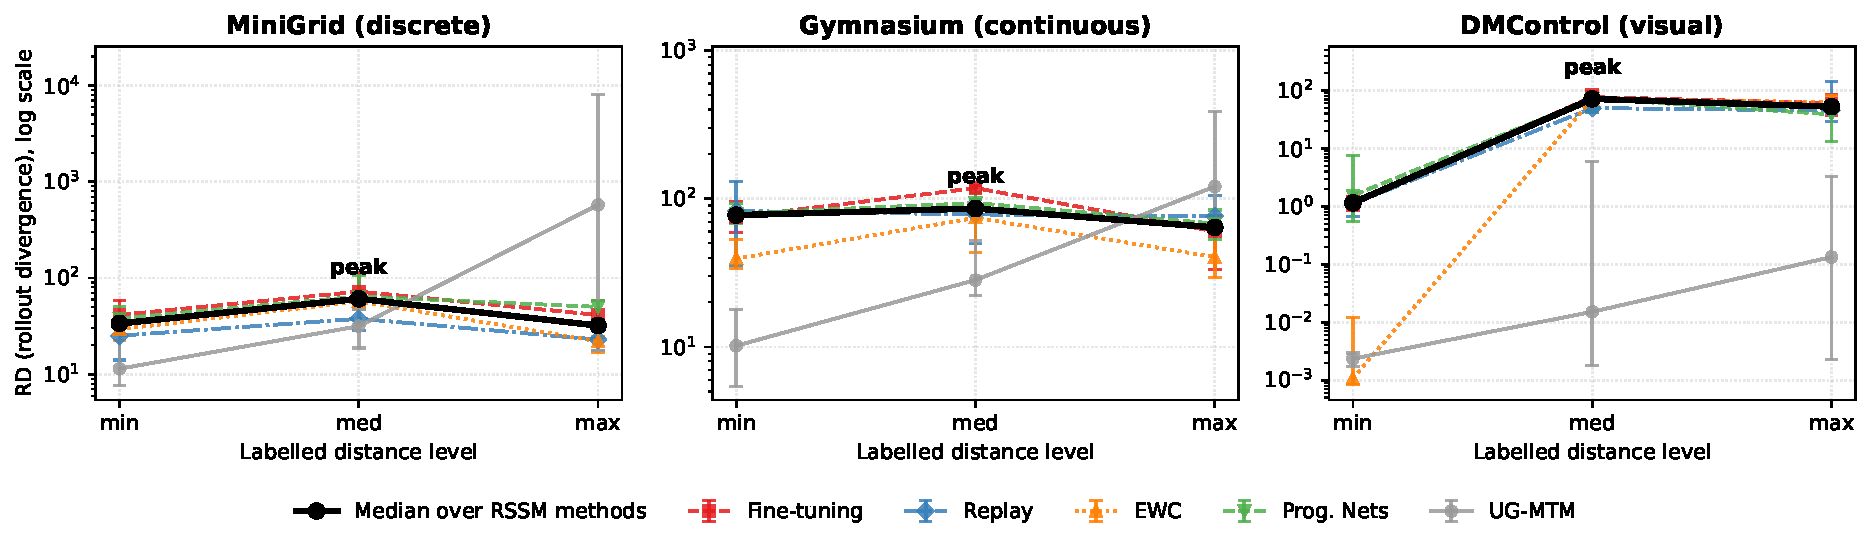
\includegraphics[width=0.72\textwidth]{axis_peak}
  \caption{Rollout divergence against the labelled distance level, one line per
  family, log scale. The peak is at the medium level in all three.}
  \label{fig:axis}
\end{figure}

\begin{table}[t]
  \centering
  % Generated by experiments/export_tables.py -- do not edit by hand.
% Regenerate after any change to results/ or to the aggregation.

\begin{tabular}{lrrrc}
\toprule
Family & min & med & max & Peak \\
\midrule
MiniGrid & 33.31 & \textbf{62.26} & 35.63 & med \\
Gymnasium & 77.45 & \textbf{85.91} & 59.59 & med \\
DMControl & 1.15 & \textbf{70.94} & 52.66 & med \\
\bottomrule
\end{tabular}

  \caption{Figure~\ref{fig:axis} as numbers: RD by family and labelled level,
  aggregated over the four methods sharing the RSSM architecture (median over
  methods of each method's median over seeds).}
  \label{tab:axis}
\end{table}

In all three families the maximum sits at the \emph{medium} level
(Figure~\ref{fig:axis}, Table~\ref{tab:axis}), so the labelled order
$\text{min} < \text{med} < \text{max}$ is wrong in every one of them. Three out
of three is the robust part of this: it does not depend on how cells are
aggregated, on which forgetting metric is read, or on any threshold.

Gymnasium makes the point without any appeal to how families compare, because
there the two upper levels are nested by construction. Both move HalfCheetah
from gravity $9.8$ to $4.0$; the maximum level additionally scales mass by $3$
and friction by $0.5$. It is strictly the medium perturbation plus more
perturbation, and it produces \emph{less} forgetting ($64.01$ against $85.91$).

The obvious objection is that this is a statement about our budget: if the
model never fits task~B at the maximum level, nothing is overwritten. We reran
both cells at twice the budget, and it does not hold up. Restricted to
fine-tuning and to the five seeds both budgets share, the cells read $118.04$
(medium) against $58.79$ (maximum) at 5000 updates and $144.70$ against
$102.18$ at 10000. The mechanism the objection proposes is backwards: task~B is
\emph{easier} to fit at the maximum level at both budgets ($17.44$ against
$27.28$, and $15.14$ against $24.65$), because the heavier, lower-friction,
low-gravity cheetah moves less, and a less varied task has less to learn from.
What is robust is the direction; the magnitude is budget-dependent, the ratio
between the two cells falling from $2.01$ to $1.42$.

\subsection{What does predict forgetting, and how far to trust it}
\label{sec:results:predictors}

\begin{table}[t]
  \centering
  % Generated by experiments/export_tables.py -- do not edit by hand.
% Regenerate after any change to results/ or to the aggregation.

\begin{tabular}{llrrr}
\toprule
Family & Level & RD & $d_{\mathrm{trans}}$ & Task-B difficulty \\
\midrule
MiniGrid & min & 33.73 & 22.35 & 2.01 \\
 & med & 60.88 & 20.64 & 42.60 \\
 & max & 32.11 & 25.19 & 23.59 \\
\addlinespace
Gymnasium & min & 77.45 & 28.75 & 24.63 \\
 & med & 85.91 & 30.86 & 27.28 \\
 & max & 64.01 & 24.08 & 17.44 \\
\addlinespace
DMControl & min & 1.15 & 1.87 & 15.43 \\
 & med & 71.64 & 7.58 & 34.07 \\
 & max & 52.61 & 7.46 & 40.54 \\
\midrule
\multicolumn{2}{l}{Spearman $\rho$ with RD} & 0.00 & 0.58 & 0.43 \\
\multicolumn{2}{l}{\quad (predictor)} & \emph{labelled level} & \emph{measured} & \emph{measured} \\
\bottomrule
\end{tabular}

  \caption{The nine cells behind the rank correlations, and the correlations.
  Task-B difficulty is the held-out reconstruction error a model reaches on
  task~B after training on it.}
  \label{tab:predictors}
\end{table}

Table~\ref{tab:predictors} compares three candidate predictors across the nine
cells: the label, the measured distance $d_{\mathrm{trans}}$, and the
difficulty of task~B. The label carries no rank information ($\rho = 0.00$).
Both measured quantities do better ($0.58$ and $0.43$), and we deliberately do
not rank them against each other: at nine cells they swap places when seeds are
added, which is itself the evidence that nine cells do not resolve them.

We read the result as forgetting scaling with what the new task demands of the
model, and state it as the best available account rather than a demonstrated
mechanism, because DMControl does not follow it --- task-B difficulty there
rises from minimum to maximum while forgetting falls after the medium level.

$d_{\mathrm{trans}}$ is not a drop-in replacement for the axis, and its leading
$\rho$ should not be read as one. Between families it separates cleanly, and
that separation is what most of the correlation is made of; \emph{within} a
family it mostly does not separate at all. Gymnasium's three levels span about
seven units in the median while individual cells span fifteen to twenty-three
across seeds, and at twice the budget its medium and maximum medians swap
places. What survives is narrower and still worth stating: a measured distance
is answerable to evidence in a way a label is not, and this one answered ---
including about itself.

\subsection{Three cells produce no forgetting, and we report them as controls}
\label{sec:results:controls}

We call a cell a \emph{control} when no method's held-out task-A reconstruction
grows by more than 10\% after training on task~B. The threshold is not a knife
edge: in every cell that does produce forgetting, the worst method ends between
$14.8\times$ and $848\times$ its original error. Three of the nine qualify:
Gymnasium at minimum and medium distance, where the task pair is the same
HalfCheetah under different gravities, and DMControl at minimum. That is what
the bottom of a distance axis should look like, and the benchmark detects it;
it also means those cells discriminate on nothing, and the effective grid is
six cells rather than nine. The criterion is deliberately blind to RD, and
Gymnasium's medium cell shows why: it loses nothing in pixels and
simultaneously carries the highest RD in its family.

\subsection{Forgetting happens in the encoder, where the metrics cannot see it}
\label{sec:results:encoder}

\begin{table}[t]
  \centering
  % Generated by experiments/export_tables.py -- do not edit by hand.
% Regenerate after any change to results/ or to the aggregation.

\begin{tabular}{llrrrrr}
\toprule
Family & Level & Fine-tuning & Replay & EWC & Prog.\ Nets & UG-MTM \\
\midrule
MiniGrid & min & 811 & 1.31 & 800 & 797 & 1.00 \\
 & med & 829 & 1.18 & 848 & 825 & 1.00 \\
 & max & 32 & 1.02 & 31 & 31 & 1.00 \\
\addlinespace
Gymnasium & min$^{\dagger}$ & 0.94 & 0.90 & 0.94 & 0.97 & 1.00 \\
 & med$^{\dagger}$ & 1.04 & 0.92 & 1.05 & 1.06 & 1.00 \\
 & max & 14 & 1.04 & 15 & 14 & 1.00 \\
\addlinespace
DMControl & min$^{\dagger}$ & 1.02 & 1.00 & 1.02 & 1.02 & 1.00 \\
 & med & 16 & 0.37 & 16 & 16 & 1.00 \\
 & max & 17 & 0.51 & 17 & 16 & 1.00 \\
\bottomrule
\end{tabular}

  \caption{Held-out task-A reconstruction error after training on task~B, as a
  factor of the same model's error before it. $1.00$ means nothing was lost.
  $\dagger$ marks control cells.}
  \label{tab:encoder}
\end{table}

Table~\ref{tab:encoder} shows the size of the blind spot that
Section~\ref{sec:benchmark} declared. Fine-tuning's held-out task-A
reconstruction grows by a factor of $811$ in MiniGrid at minimum distance while
its PF for that cell is $-5.58$: measured in the frozen latent basis, the model
\emph{improved}. This is not an isolated sign error --- fine-tuning's PF is
negative in eight of the nine cells while its encoder is destroyed in six.

EWC makes the dissociation sharpest, and it was derived before it was measured.
Its Fisher information is defined over $\log P(z' \mid z, a)$, in which no
encoder parameter appears, so its entries there are \emph{exactly} zero and the
quadratic penalty cannot constrain them even in principle. Both halves hold:
EWC preserves the transition component almost perfectly ($-0.03$) while its
encoder degrades by a factor of $800$, marginally worse than the unregularised
baseline. Replay is the only method that keeps both, its task-A reconstruction
never growing by more than $27\%$.

The lesson generalises past our metrics: \textbf{any latent-space forgetting
metric evaluated on frozen representations measures the component it was
pointed at and reports nothing about the representation}, and in an end-to-end
world model the representation is where most of the damage is. Recording a
representation-space quantity alongside costs one forward pass per evaluation.

\subsection{What the benchmark says about the methods}
\label{sec:results:methods}

Read across both scales the three strategies separate, and none dominates.
\textbf{Replay} keeps both components and has the lower RD in five of the six
cells that produce forgetting, four of them unanimously across ten seeds
($p = 0.002$, $d_z$ from $-2.28$ to $-3.11$); it is worse in one (Gymnasium at
maximum, $p = 0.006$, $d_z = +1.14$) and indistinguishable in another
($p = 0.68$). It pays where it works hardest, with the worst forward transfer
of the four RSSM methods in the cells where it best protects the encoder ---
though replay trains on A and B together, so half its gradient steps go to
task-A data and its FT confounds transfer with a halved budget on B.
\textbf{Regularisation} protects what its penalty covers and nothing else, as
above. \textbf{Structural isolation}, ours included, buys preservation by
declining to learn: our method's task-A reconstruction is unchanged to the bit
in all nine cells, because its encoder is frozen, and it pays in forward
transfer by two orders of magnitude more than any other method. Freezing has a
second consequence we did not anticipate: the post-B transition models become
overconfident, with some latent dimensions collapsing to $\sigma = 0.007$ and
the rollout KL already at $80$ at step~0. Confident and wrong is a failure mode
an unbounded divergence surfaces and a mean hides.

\section{Discussion}
\label{sec:discussion}

\subsection{What ``controlled dynamic distance'' can and cannot mean}

What is genuinely controlled is the \emph{construction}, and in Gymnasium in
the strongest sense available: the maximum level is the medium perturbation
plus two further ones on the same task pair. If the axis ordered anything
monotone, a strict superset could not come out below. What is not controlled is
the quantity the label is taken to stand for, and the ordering of the labels
survives contact with neither of the two things we can measure. A label that
neither predicts the outcome nor tracks the measured construct is a name, not a
control.

The recommendation is narrow and cheap: \textbf{report a measured distance for
every task pair and treat level labels as construction parameters rather than
as an independent variable.} $d_{\mathrm{trans}}$ costs one model per
environment --- a 20\% surcharge on our training budget --- and is defined
wherever transitions can be sampled. It is not a finished instrument, as
Section~\ref{sec:results:predictors} reports of our own, but it is measured,
comparable, and answerable.

\subsection{Two things called ``distance'' are being conflated}

The peak at the medium level repeats across families, which invites a mechanism
rather than a list of exceptions. The one we favour, and cannot yet establish,
is that forgetting tracks \emph{how much the model actually updates}, and that
this is non-monotone in distance for a reason unrelated to similarity: at
minimum distance there is little to update, and at maximum distance the model
often fails to fit task~B at all. Overwriting needs a task that is both
different and learnable.

If that is right, task distance bundles two variables that come apart.
\emph{Dissimilarity} is how far the new dynamics sit from the old.
\emph{Learning demand} is how much the model must change to fit the new task at
the available budget. They correlate at the low end and decouple at the high
end, where a distant task can be too hard to learn from. That is why a single
scalar predictor reaches $0.58$ and not higher, and why DMControl breaks the
account: there difficulty has stopped meaning ``much to learn'' and started
meaning ``too hard to learn''. Separating them needs a predictor built from
what the optimiser did during task~B rather than from the outcome, which we did
not run.

\subsection{What the encoder result asks of benchmark design}

EWC's zero is worth stating generally: \textbf{the protected set is exactly the
support of whatever likelihood the Fisher is estimated from}, and in modular
architectures that support is usually narrower than the module list suggests.
The failure is invisible to any metric sharing the same restriction --- which,
in our first formulation, was every metric we reported. A component-level
benchmark that reports only its component-level metric can certify the
preservation of a system that has been substantially destroyed.

\subsection{Limitations}
\label{sec:discussion:limitations}

The binding constraint is statistical resolution: at ten seeds the exact paired
test floors at $p \approx 0.002$, and the three control cells remain at five,
where the floor is $0.0625$. The grid is nine cells of which six discriminate,
and one architecture family --- every method here is a variation on the same
recurrent latent world model, so the results speak to that class. The
experiments reported here run \emph{one} task switch, which is a thin reading of
``continual''; a four-task MiniGrid sequence, reported in full elsewhere, shows
the same intermediate peak along sequence position rather than a monotone
increase, but that is one family and one sequence. The budget
(20 random-policy episodes per task, 5000 updates, latent dimension 32) is
small enough that absolute magnitudes are budget-dependent, though task~A is
demonstrably learned at this scale and the central finding survives doubling
it. Task-B difficulty and RD are computed from the same runs, so a cell with
hard data inflates both; this is not circular but admits the reading ``this
cell is hard''. Finally, the prediction that distinguishes our account from the
design's is cheap and untested: forgetting should fall again at distances large
enough that task~B stops being learnable at the given budget.

\section{Conclusion}
\label{sec:conclusion}

We built a benchmark to ask which continual learning method best preserves a
world model's transition component, and the two things it told us are about the
question rather than the answer. The distance axis it was designed around does
not order forgetting in any of three families, and the label carries no rank
information across the nine cells; what forgetting tracks is closer to what the
new task demands than to how far it sits from the old. And the forgetting is
concentrated in the encoder, where component-level metrics --- ours included
--- are blind by construction, so a suite reporting only them would certify the
preservation of models whose representation had been destroyed
eight-hundred-fold. Both results are cheap to act on: report a measured
distance per task pair and hold it to account, and report a
representation-space quantity beside the component-level one. We characterise
five methods rather than ranking them, our own among them and not favourably.

\subsubsection*{Reproducibility}

Code, configurations, the table-generating scripts and all 375 result files are
released. Every table here is generated from the stored results rather than
transcribed; the protocol is declared in configuration, recorded in every
result file, and the runner refuses to combine results produced under different
ones. A cell re-executed eight days after its original run reproduced to the
fourth decimal.

\bibliographystyle{plainnat}
\bibliography{refs}

\end{document}
